\documentclass{standalone}

\usepackage{circuitikz}

\begin{document}
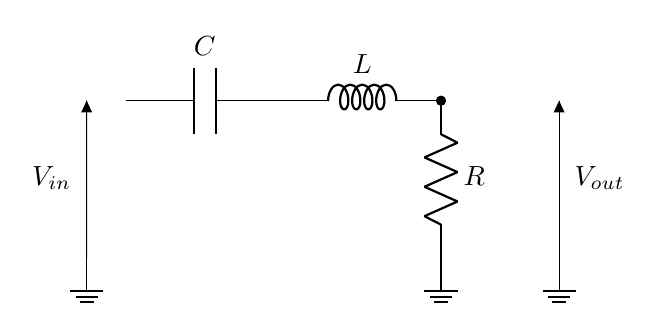
\begin{tikzpicture}
	\draw (0,0) 
	to[C, l=$C$,-] (2,0) 
	to[L, l=$L$, -*] (4,0) 
	to[R, l=$R$, *-] (4,-2) 
	to[short](4,-2)   node [ground] {};
	%input
	\draw (-0.5,0)
	to[short, l_=$V_{in}$](-0.5,-2)   node [ground] {};
	\draw (-0.5,0) coordinate[inputarrow,rotate=90];
	% output
	\draw (5.5,0)
	to[short, l=$V_{out}$](5.5,-2)   node [ground] {};
	\draw (5.5,0) coordinate[inputarrow,rotate=90];
\end{tikzpicture}
\end{document}